\section{Pretraživanje penjačkih lokacija, sektora, penjačkih lokacija i korisnika}

Kako bi korisnici mogli brzo pronaći informacije, aplikacija omogućuje pretraživanje penjačke lokacije, sektora, penjačkih smjerova i korisnika. Pristupom zaslonu za pretraživanje, korisnik se prikazuje trenutna traka za unos teksta te, inicijalno, popis nedavno pregledanih stavki, što omogućuje brz povratak na prethodno pregledane elemente.

\begin{figure}[H]
    \centering
    \begin{subfigure}[b]{0.48\textwidth}
        \centering
        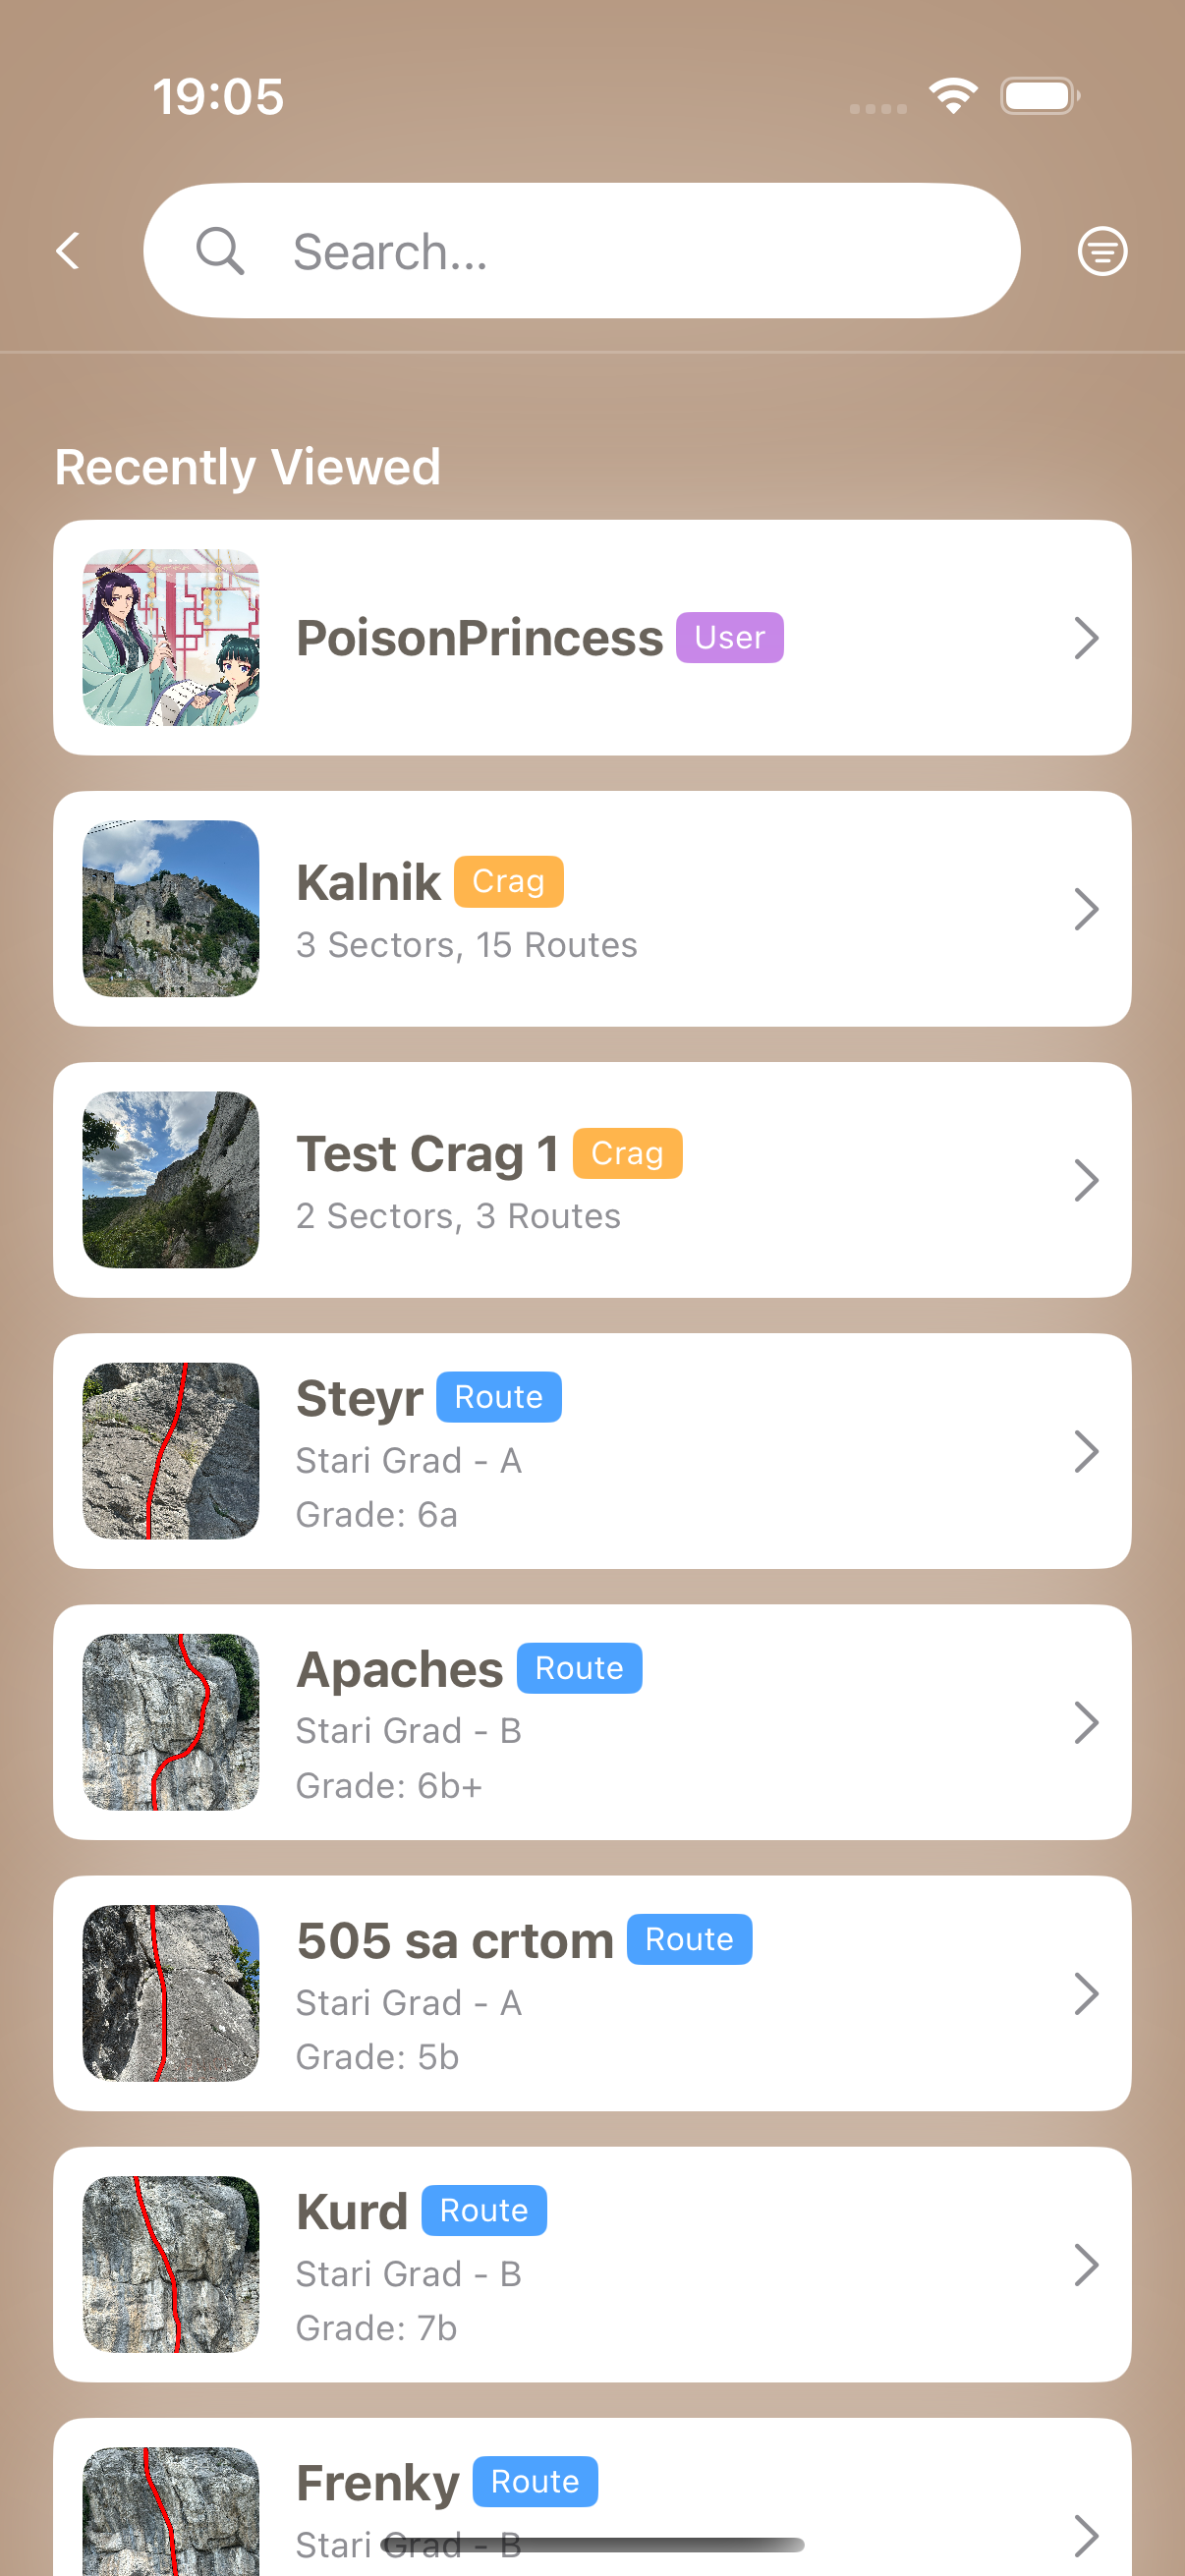
\includegraphics[width=\textwidth]{images/implementacija/search_default.png}
        \caption{Početno stanje pretraživanja}
        \label{fig:pretrazivanje_default}
    \end{subfigure}
    \hfill
    \begin{subfigure}[b]{0.48\textwidth}
        \centering
        
\includegraphics[width=\textwidth]{images/implementacija/search_searching.png}
        \caption{Pretraživanje s unesenim pojmom}
        \label{fig:pretrazivanje_searching}
    \end{subfigure}
    \caption{Pretraživanje penjačkih lokacija, sektora, penjačkih smjerova i korisnika}
    \label{fig:pretrazivanje_sidebyside}
\end{figure}

Sustav pretraživanja je dinamičan i reagira na korisnikov unos. Upisivanjem pojma u traku za pretraživanje, aplikacija filtrira popis dostupnih penjačkih lokacija, sektora, penjačkih smjerova i korisnika te prikazuje relevantne rezultate iz više kategorija istovremeno. Svaki rezultat pretrage prikazan je u obliku pregleda kartica koja sadrži informacije poput naziva i tipa sadržaja, te dodatne podatke ovisno o tipu sadržaja. Penjačke lokacije sadrže broj sektora i penjačkih smjerova, sektori broj penjačkih smjerova, a korisnici broj penjačkih smjerova koje su popeli. Odabirom bilo kojeg rezultata, korisnik se preusmjerava na odgovarajući detaljni prikaz. 

Funkcionalnosti pretraživanja na web aplikaciji su iste kao i na mobilnoj aplikaciji. Pretraživanje je moguće pristupiti klikom na sekciju pretraživanja u gornjem desnom kutu stranice. Na prvoj stranici taj element se nalazi u centru stranice. Također je moguće pristupiti tipkovnim prečcom pritiskom gumba CTRL na tipkovnici i slovom k.

\begin{figure}[H]
    \centering
    \begin{subfigure}[b]{0.48\textwidth}
        \centering
        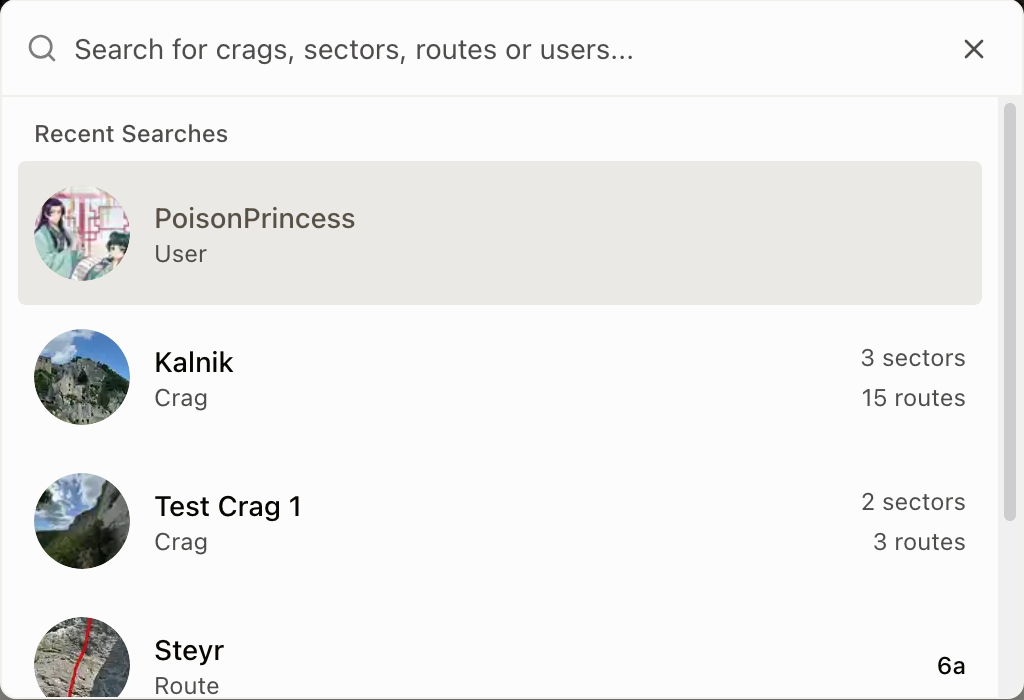
\includegraphics[width=\textwidth]{images/implementacija/web/search_default.png}
        \caption{Početno stanje pretraživanja na web aplikaciji}
        \label{fig:pretrazivanje_web_1}
    \end{subfigure}
    \hfill
    \begin{subfigure}[b]{0.48\textwidth}
        \centering
        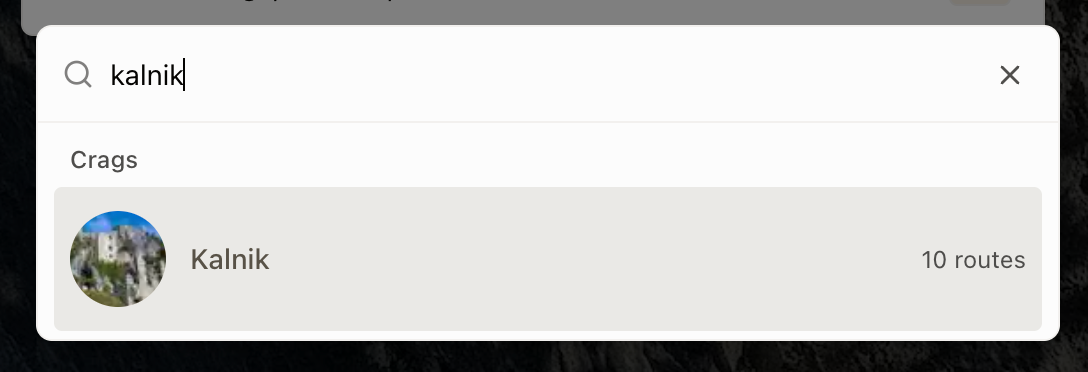
\includegraphics[width=\textwidth]{images/implementacija/web/search_searching.png}
        \caption{Traženje na web aplikaciji}
        \label{fig:pretrazivanje_web_2}
    \end{subfigure}
    \caption{Funkcionalnost pretraživanja na web aplikaciji}
    \label{fig:pretrazivanje_side_by_side}
\end{figure}